\section{Аналогові датчики}

\textbf{NTC терморезистор}\bigskip

Терморезистор, за своєю суттю резистор, який зроблений з напівпровідника та змінює свій опір зі зміною температури. Можна визначити два типи терморезисторів -- NTC терморезистор (термістор), який зменшує опір при нагріві (саме про них піде далі), та PTC терморезистор (позистор), який збільшує опір при нагріві. Є досить багато типів терморезисторів за формфактором, їх можна побачити на рис.~\ref{fig:thermoresistor_types}.

\begin{figure}[ht]
    \centering
    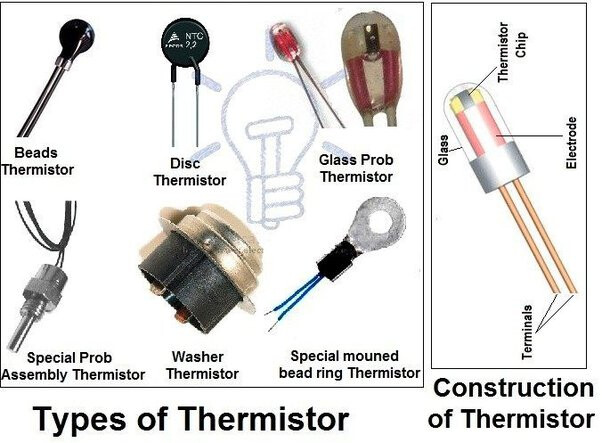
\includegraphics[width=0.7\linewidth]{thermoresistor_types.jpg}
    \caption{Різні типи терморезисторів}
    \label{fig:thermoresistor_types}
\end{figure}

На невеликому проміжку залежність опору від температури є лінійною, що дозволяє виконати апроксимацію використовуючи температурний коефіцієнт опору (TCR) для цієї області, та знаючи для якої референсної температури він відноситься (наприклад $25^\circ~C$) (рівняння \ref{eq:tcr}).

\begin{equation}
    \label{eq:tcr}
    \rho = \rho_0\left(1+\alpha\frac{t-t_0}{t_0}\right)
\end{equation}

На усьому робочому діапазоні залежність вже не лінійна, а отже розрахунки по такій формулі дадуть досить високу похибку на границях діапазону (рис.~\ref{fig:ntc_curve}).

\begin{figure}[ht]
    \centering
    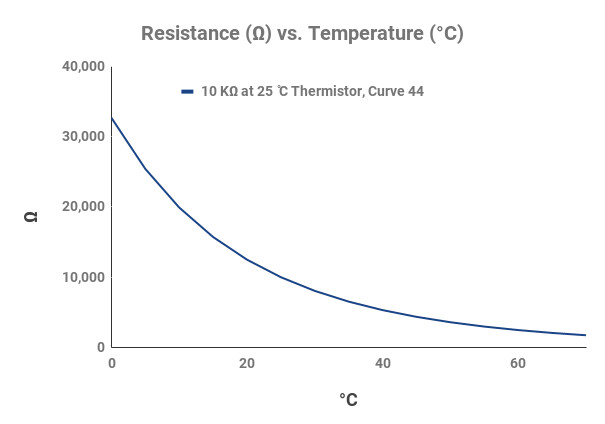
\includegraphics[width=0.9\linewidth]{ntc_curve.jpg}
    \caption{Характеристика NTC термістора}
    \label{fig:ntc_curve}
\end{figure}

Для деяких термісторів можна знайти специфікацію, у якій може бути надана таблиця залежності температури від опору з кроком 1°C або 5°C, проміжні значення можна розрахувати використовуючи лінійну інтерполяцію.

Зазвичай використовують іншу формулу для розрахунку температури з опору. Одним з параметрів, що характеризують залежність опору від температури, є коефіцієнт температурної реакції, що позначається $B$ та вимірюється у кельвінах. Цей коефіцієнт розраховується зі значень опору при двох конкретних температурах, і для багатьох термісторах може бути від 2600 до 4200K. У багатьох випадках ці температури вибирають 25°C і 100°C. Як правило, температури, використовувані при розрахунку коефіцієнта, задаються після букви, наприклад B25/100. Наступна експоненційна формула \ref{eq:ntc_beta} може бути використана для більш точних розрахунків.

\begin{equation}
    \begin{aligned}
        \text{R}_t = \text{R}_0 e^{\beta\left(\frac{1}{T}-\frac{1}{T_0}\right)}
        & \text{ , де T -- температура термістора} \\
        & \text{$T_0$ -- референсна температура} \\
        & \text{$\text{R}_0$ -- опір при референсній температурі} \\
        & \text{$\beta$ -- коефіцієнт температурної реакції}
    \end{aligned}
    \label{eq:ntc_beta}
\end{equation}

Окрім цього можна скористатися формулою Стейнхарта-Харта, яка дозволяє ще точніше розраховувати температуру, знаючи A, B, C коефіцієнти для взятого термістора (часто є у специфікації).

\begin{equation}
    \begin{aligned}
        \frac{1}{\text{T}} = A + B\ln(\text{R}) + C\left[\ln(\text{R})\right]^3
        & \text{ , де T -- температура у Кельвінах} \\
        & \text{R -- опір резистора}
    \end{aligned}
\end{equation}

\begin{figure}[ht]
    \centering
    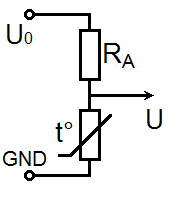
\includegraphics{ntc_connect.jpg}
    \caption{Схема підключення термістора}
    \label{fig:}
\end{figure}

Висновки по NTC термістру:

\begin{itemize}
    \item Сам по собі термістор має високу точність та малий час реакції, але без належного калібрування значення температури будуть відрізнятися на декілька градусів (особливо при зменшенні температури);
    \item Розрахунок температури можна зробити декількома способами: використовуючи рівняння, що на деяких мікропроцесорах буде сповільнювати роботу програми, або табличним способом, коли розраховуються значення температур в залежності від опору з деяким кроком, а проміжні значення отримуються за допомогою лінійної інтерполяції;
    \item Термістор вмикається в схему у верхнє або нижнє плече дільника напруги (від цього залежатиме вид характеристики). Зміна опору термістора призводить до зміни напруги дільника;
    \item Обираючи номінали дільника (резистора і термістора), слід врахувати, що струм, який протікає через термістор, спричиняє його нагрівання і, як наслідок, спотворення показань;
    \item Термістор один з найдешевших датчиків температури, що є великою перевагою.
\end{itemize}

\textbf{Термопара К-типу}\bigskip

Основною перевагою термопар є їх широкий температурний діапазон. Обмежена, по суті, абсолютним нулем (з нюансами) і температурою плавлення металів, тобто здатна робити виміри, де інші датчики просто вийдуть зі стану -- від -270 до + 1800$^\circ$C і вище.

Термопара досить цікавий датчик, адже в ній використовується інший ефект -- ефект Зеєбека, і на відміну від термістора, вона є пасивним датчиком, тобто створює дуже низьку напругу в залежності підвищення температури. Тут потрібно з'ясувати як саме вона працює.

Річ у тому, що при з'єднанні двох різнорідних сплавів провідників (наприклад Алюмель та Хромель) при їх нагріванні виникає різниці потенціалів, яка і генерує напругу. Нагрівати ми будемо так званий ``гарячий'' сплав, і зчитувати його напругу. Тут важливо зауважити, що інший -- ``холодний'' сплав, не можна нагрівати, адже саме при різних температурах виникає Електрорушійна сила, яка прямо пропорційно різниці цих температур. Термопара це відносний датчик, тому температура зовнішнього середовища до уваги не береться, важливі тільки відносини двох сплавів.

Як можна було зрозуміти, на виході (після перетворення) ми отримаємо температуру відносно холодного сплаву, а отже, щоб отримати реальну температуру на гарячому сплаві, потрібно завчасно виміряти температуру на холодному (референсному), для цього можна використати той же термістор. Цікаво, що цю проблему можна також вирішити помістивши холодний сплав у воду температури $0^\circ~C$, тоді компенсувати значення з гарячого сплаву не потрібно.

В залежності від потреб використовуються різні сплави, наприклад наша термопара К-типу використовує Алюмель (холодний) та Хромель (гарячий), і дозволяє вимірювати у досить широкому діапазоні, з кінцевими границями у $-200^\circ~C$ -- $1260^\circ~C$, таку термопару зручно використовувати для термостата у паяльні станції. Термопара Е-типу складається з Хромелю та Константану, і дозволяє вимірювати дуже низькі температури, не піддається корозії, і тому може бути використана у вологих середовищах. Також використовуються наступні сплави: E (хромель-константант), J (залізо-константант), K (хромель-алюмель), M (мідно-копель), N (ніхросил-нісил) та інші.

Як було сказано вище, термопара генерує низьку напругу, К-типу -- 0.4мВ/$^\circ$C, АЦП з роздільною здатністю 10 бітів не здатен зчитати таку напругу, тому її потрібно спочатку підсилити за допомогою неінвертуючого підсилювача, про це більш детально у практичній частині.

Для перетворення значення з підсиленого виходу термопари у температуру скористуємося наступною формулою \ref{eq:thermocouple}.

\begin{equation}
    \label{eq:thermocouple}
    \begin{aligned}
        T = \frac{V}{Ga} + T_{\text{ref.}}
        & \text{ , де V -- підсилений сигнал} \\
        & \text{G -- коефіцієнт підсилення} \\
        & \text{$\alpha$ -- коефіцієнт Зеєбека, табличне значення} \\
        & \text{$T_{\text{ref.}}$ -- температура холодного сплаву}
    \end{aligned}
\end{equation}

\begin{figure}[ht]
    \centering
    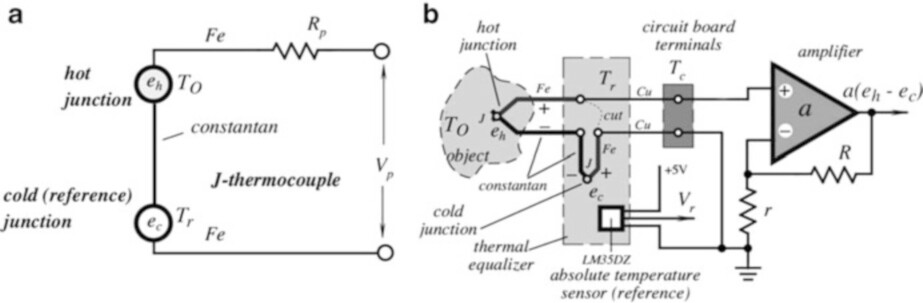
\includegraphics[width=\linewidth]{thermocouple_usage.jpg}
    \caption{Приклад використання термопари}
    \label{fig:thermocouple_usage}
\end{figure}
%\FloatBarrier

Висновки по термопарі К-типу:

\begin{itemize}
    \item Більше ніяких складних формул, у термопарі К-типу ми маємо лінійну залежність 0.4мВ/$^\circ$C вище нуля, все що потрібно це підсилити цю напругу та скористатися простою формулою;
    \item Термопара має нижчу швидкість реакції, а той же час здатна вимірювати високі температури;
    \item Має непогану точність, але її складно досягти, без ізоляцій і фільтрів на входах та виходах. Термопара К-типу має майже лінійну залежність, тому калібровка не є складно. Ці нюанси не такі вже і важливі, адже термопарою вимірюють високі температури, де похибка у декілька градусів не страшна.\\
\end{itemize}
